\documentclass[12pt]{article}

\usepackage{graphicx}
\usepackage{paralist}
\usepackage{amsfonts}
\usepackage{hyperref}
\usepackage{listings}
\usepackage{subfig}
\usepackage{float}

\oddsidemargin 0mm
\evensidemargin 0mm
\textwidth 160mm
\textheight 200mm
\renewcommand\baselinestretch{1.0}

\pagestyle {plain}
\pagenumbering{arabic}
\newcounter{stepnum}

\title{Course Project}
% \author{Hyosik Moon}
\author{
  Moon, Hyosik
  }

\begin {document}

\maketitle

\section{Required}

\begin{itemize}
\item \textbf{Main objective of the analysis} \\
Predict next-day rain by training classification models on the target variable RainTomorrow. We will predict the next-day rain by using three different models such as Logistic Regression, Support Vector Machine (SVM), and Random Forest with cross validation. And analyze the models accuracy and coefficients to find the impactful features.

\item \textbf{Brief description of the data set} \\
This dataset contains about 10 years of daily weather observations from many locations across Australia. RainTomorrow is the target variable to predict. This column is Yes if the rain for that day was 1mm or more. In data set, there are 23 columns and there are 16 floats and 7 objects columns. \ref{data_info}

\begin{figure}[H]
    \centering
    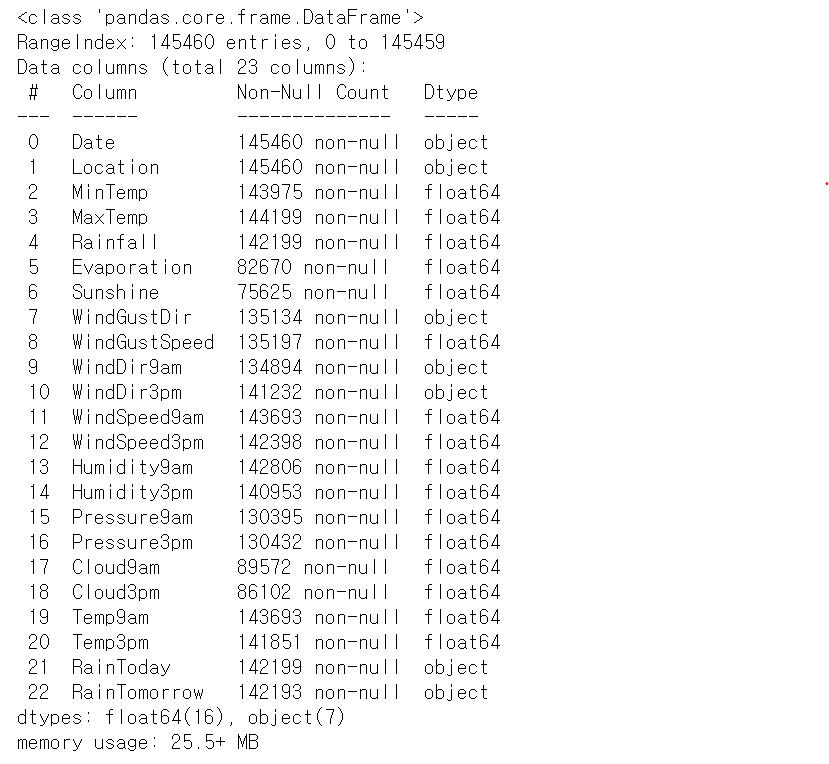
\includegraphics[width=0.9\textwidth]{figures/data_info.png}
    \caption{Data set information}\label{data_info}
\end{figure}

\item \textbf{Brief summary of data exploration}
    \begin{enumerate}
    \item Data cleaning. First, delete NaN data. Second, delete unused features (columns). We can delete Date column but it can be useful if we use `month' to predict the RainTomorrow. So, we will change the Date column to month rather than delete the column.
    \item Correlation. To see the correlation, we have to change categorical variables to numeric variables. So, let's change the objects to numeric by using LabelEncoder. Find the correlation between RainTomorrow and other features (Figure \ref{corr}, \ref{corr2}). We don't know what is the most impactful feature to predict RainTomorrow even though we can refer to the correlation. So, before we find the important features, we will use the all features.
    
    \begin{figure}[H]
      \centering
      \subfloat[Correlation]{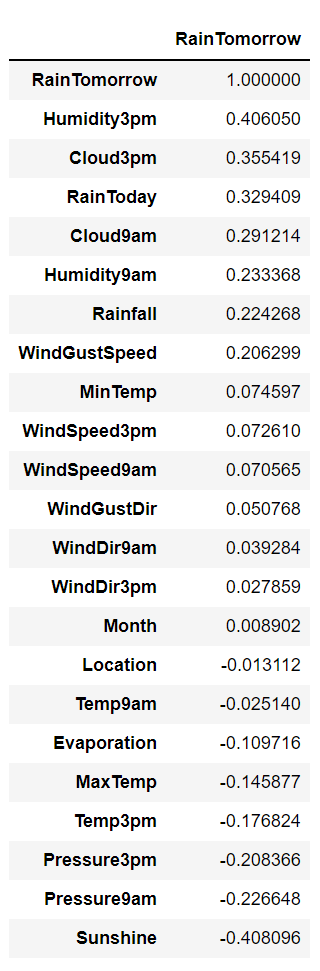
\includegraphics[width=0.3\textwidth]{figures/corr.png}\label{corr}}
      \hfill
      \subfloat[Correlation bar plot]{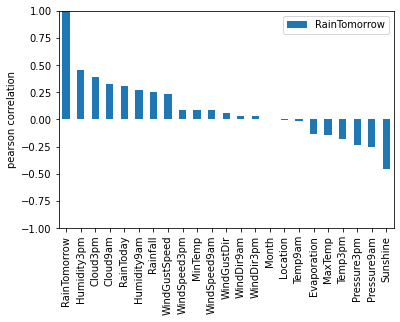
\includegraphics[width=0.65\textwidth]{figures/corr2.png}\label{corr2}}
    \end{figure}

    \item Scaling. We also need to scale the features to use the Logistic Regression and SVM. So, we will use MinMaxScaler.

    \begin{figure}[H]
      \centering
      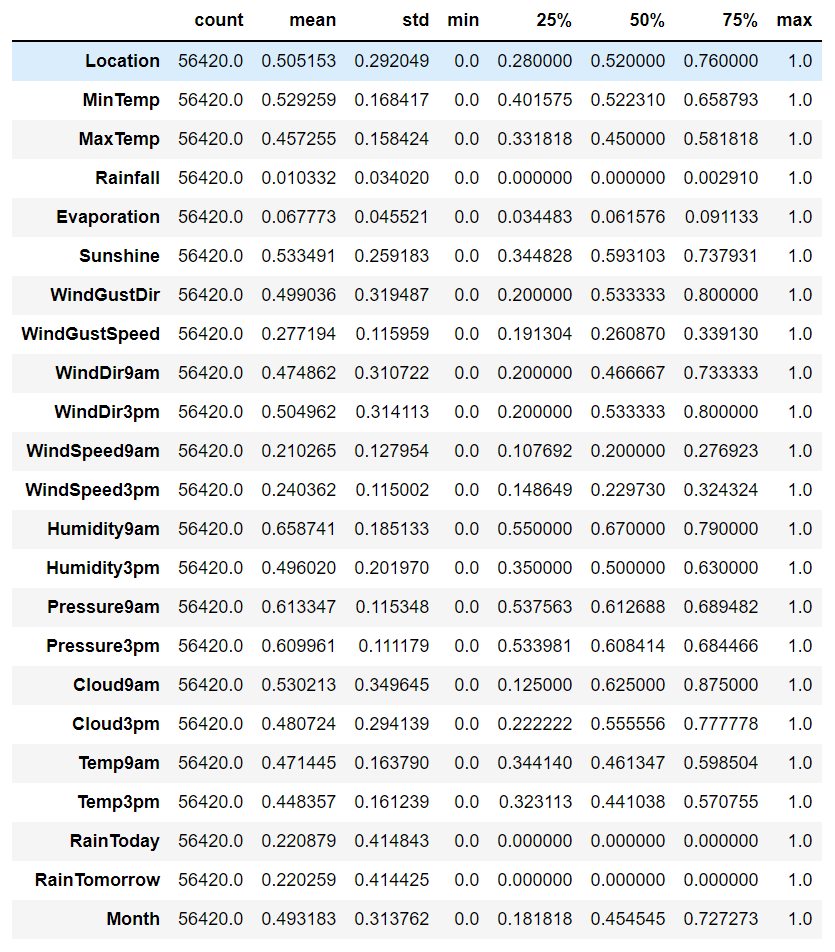
\includegraphics[width=0.8\textwidth]{figures/scaling.png}
      \caption{MinMaxScaling}\label{scaling}
    \end{figure}
    
    \end{enumerate}

\item \textbf{Summary of training at least three linear regression models} I implemented three different prediction models which are Linear Regression, Support Vector Machine, and Random Forest. And in order to regularize the models I also used cross validation.
    \begin{enumerate}
      \item LinearRegressionCV. The weighted f1-score and accuracy of the model were 0.846, 0.855 respectively. I trained the model by using stratified shuffle split because the target was skewed to 0 (No rain) (Figure \ref{lr_l1}, \ref{lr_l1_cm}).
    \end{enumerate}

    \begin{figure}[H]
      \centering
      \subfloat[Evaluation metrics for LRCV]{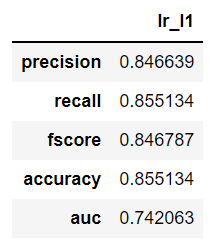
\includegraphics[width=0.4\textwidth]{figures/lr_l1.png}\label{lr_l1}}
      \hfill
      \subfloat[Confusion metrics]{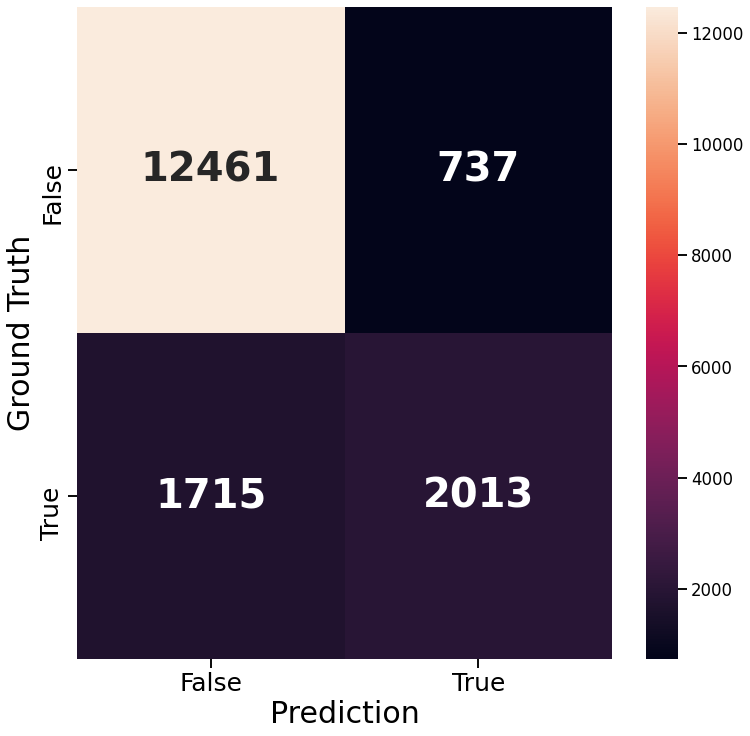
\includegraphics[width=0.5\textwidth]{figures/lr_l1_cm.png}\label{lr_l1_cm}}
    \end{figure}

    \item Support Vector Machine. The weighted f1-score and accuracy of the model were 0.846, 0.858 respectively. As a kernel function, I used rbf (Radial Basis Function) (Figure \ref{svmg}, \ref{svmg_cm}).

    \begin{figure}[H]
      \centering
      \subfloat[Evaluation metrics for SVM\_Gaussian]{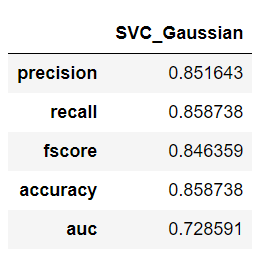
\includegraphics[width=0.4\textwidth]{figures/svmg.png}\label{svmg}}
      \hfill
      \subfloat[Confusion metrics]{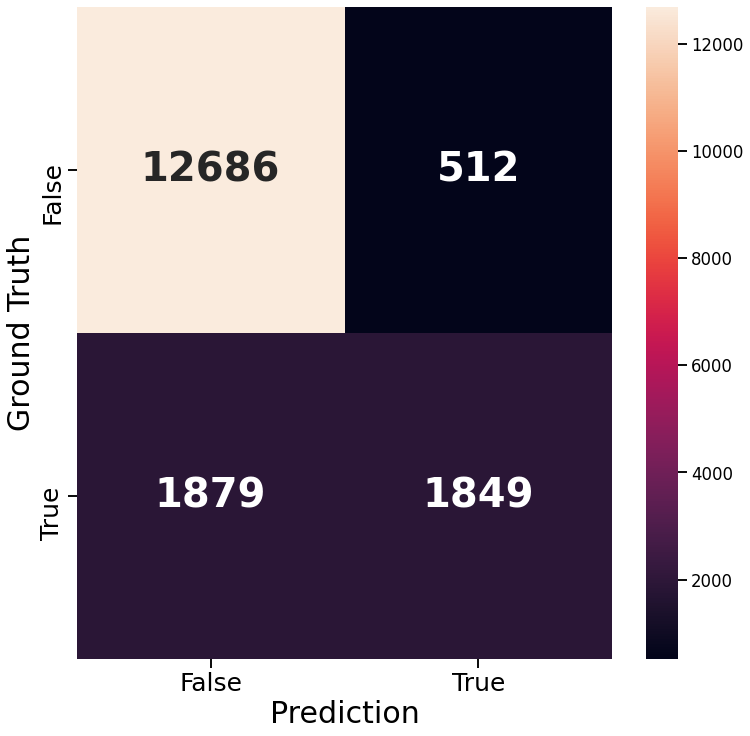
\includegraphics[width=0.5\textwidth]{figures/svmg_cm.png}\label{svmg_cm}}
    \end{figure}

    \item Random Forest. The weighted f1-score and accuracy of the model were 0.854, 0.864 respectively, and to find the best number of trees, out-of-error scores were used. And then the model use the 400 trees to predic the RainTomorrow (Figure \ref{rf}, \ref{rf_cm}, \ref{rfe}).

    \begin{figure}[H]
      \centering
      \subfloat[Evaluation metrics for Random Forest]{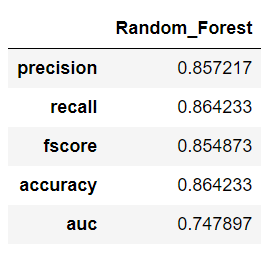
\includegraphics[width=0.4\textwidth]{figures/rf.png}\label{rf}}
      \hfill
      \subfloat[Confusion metrics]{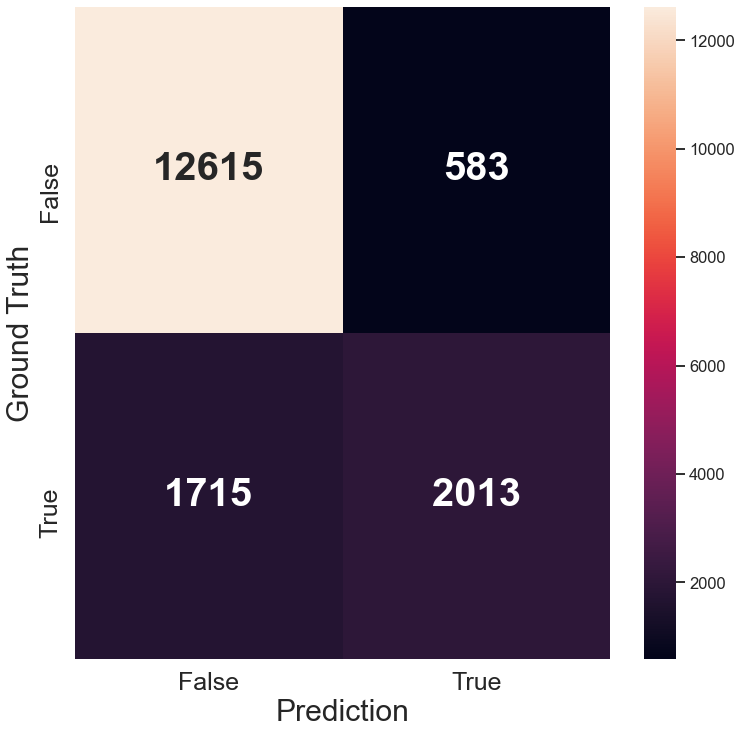
\includegraphics[width=0.5\textwidth]{figures/rf_cm.png}\label{rf_cm}}
    \end{figure}

    \begin{figure}[H]
      \centering
      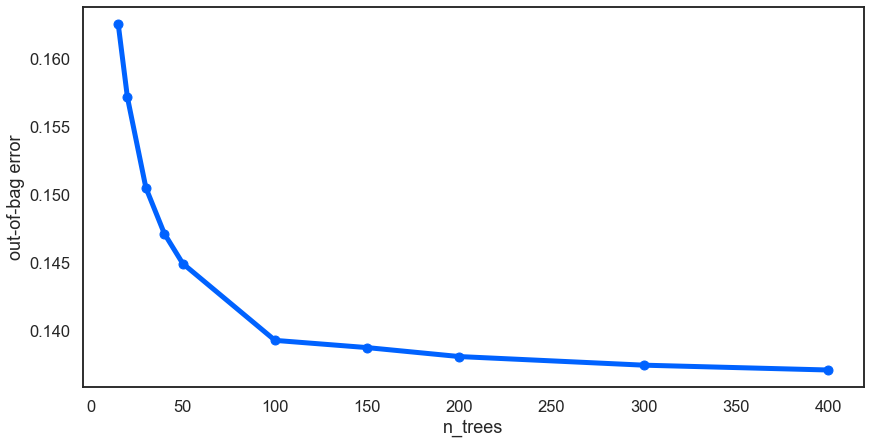
\includegraphics[width=0.8\textwidth]{figures/rfe.png}
      \caption{Out of error scores}\label{rfe}
    \end{figure}

\item \textbf{Explanation of your final regressions model}
Overall, all models showed the similar f1-score and accuracy. The best one was Random Forest which has the fscore	0.854873 and accuracy	0.864233. The ROC, Precision\_Recall curve accuracies aren't quite ideal.
This is because the RainTomorrow is unbalanced. For example, `No (rain)' takes about 77\%, `Yes (rain)' takes about 23\%. As a result the model predict the RainTomorrow relatively close to `No (rain)' even though the ground truth is `Yes (rain)'. It leads to relatively low ROC and Precision\_Recall curve accuracies (Figure \ref{roc_pr}).

\begin{figure}[H]
  \centering
  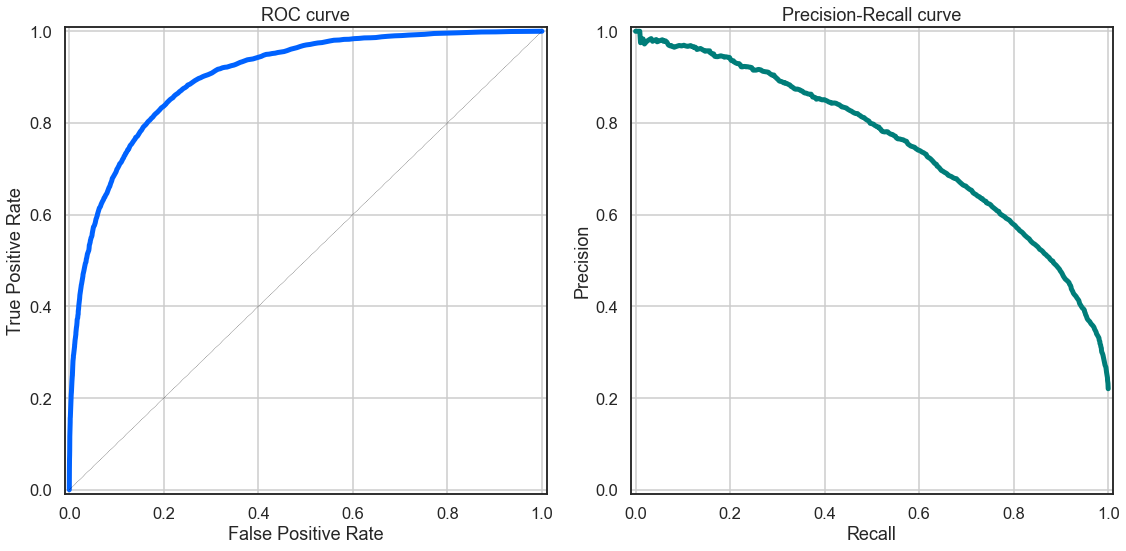
\includegraphics[width=0.8\textwidth]{figures/roc_pr.png}
  \caption{ROC, Pricision-Recall curves}\label{roc_pr}
\end{figure}

\item \textbf{Summary Key Findings and Insights}
The fact that the accuracies among the models are similir means that the reliability of the models is also high. And the three most important features to predic the RainTomorrow are `Hymidity3pm, Sunshine, and Pressure3pm'. These features are similir to the features that had high correlation values (Figrue \ref{imp}). As a result, we can conclude that `Hymidity3pm, Sunshine, and Pressure3pm' are the most important factores to predict the tomorrow's rain and with more features we can predict the tomorrows rain with 86\% accuracy.

\begin{figure}[H]
  \centering
  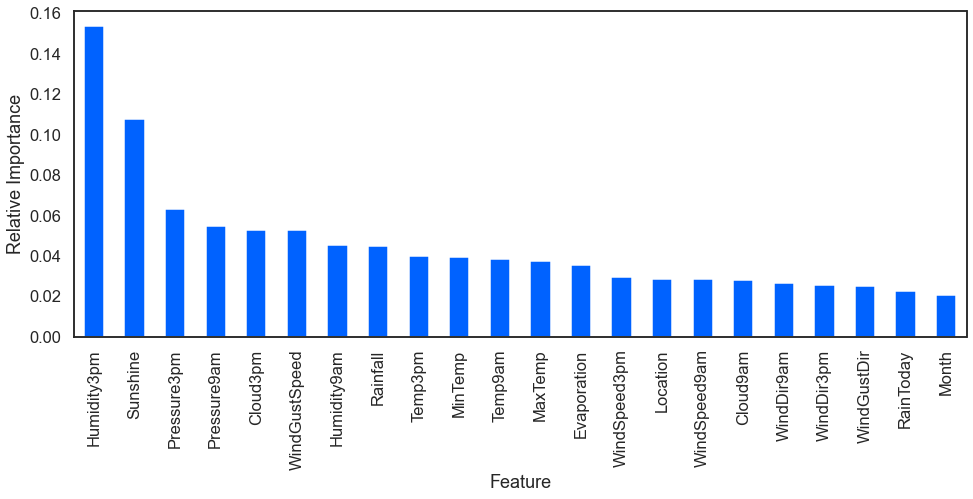
\includegraphics[width=0.8\textwidth]{figures/feature_imp.png}
  \caption{Feature importance}\label{imp}
\end{figure}

\item \textbf{Suggestions for next steps}
If the data were balanced, then we might predict more accuracte data. So, manipulating the unbalanced data will be a good-next step to imporve the model.

\end{itemize}

\end {document}